\chapter{Bedienungsanleitung}\label{bedienungsanleitung}
\section{Installation der Software}
Eclipse Installationsdialog öffnen: Menu Help / Install New Software
 \begin{figure}[H]
  	\centering
    	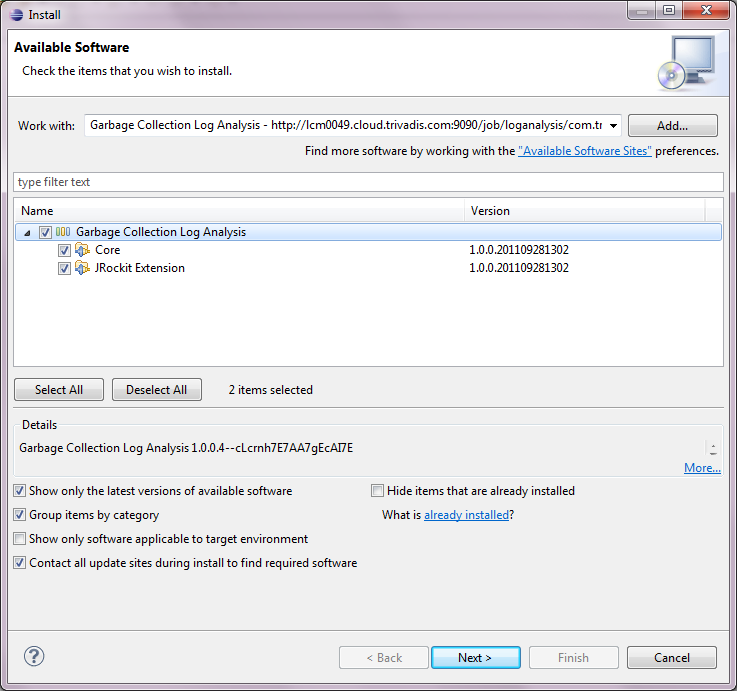
\includegraphics[width=10cm]{images/tutorial_install01}
        	\caption{Installation Garbage Collection Log Analyse}
\end{figure}
Unter Angabe der Software Update-Seite beide Features auswählen und mit zweimaligem Klick auf Next und Bestätigen der Lizenzbestimmungen installieren. Anschliessend muss die Entwicklungsumgebung neu gestartet werden.


\section{Update}
Sobald ein Update der Software via Update-Seite verfügbar ist, kann via Help / Check for Updates das Update-Fenster geöffnet werden. Die neuen updates können hier heruntergeladen und installiert werden.
 \begin{figure}[H]
  	\centering
    	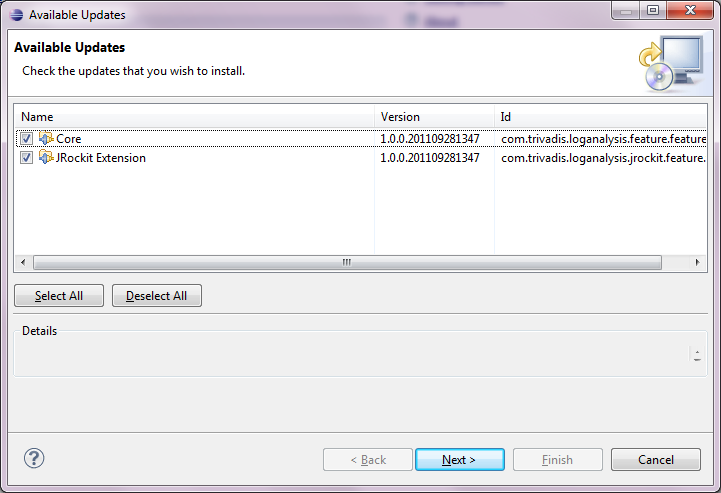
\includegraphics[width=10cm]{images/tutorial_update01}
        	\caption{Update Garbage Collection Log Analyse}
\end{figure}

\section{Dashboard}
Sobald die Software installiert ist, kann über die Toolbar und über den Knop GC Log Analysis Dashboard das Dashboard geöffnet werden. 
 \begin{figure}[H]
  	\centering
    	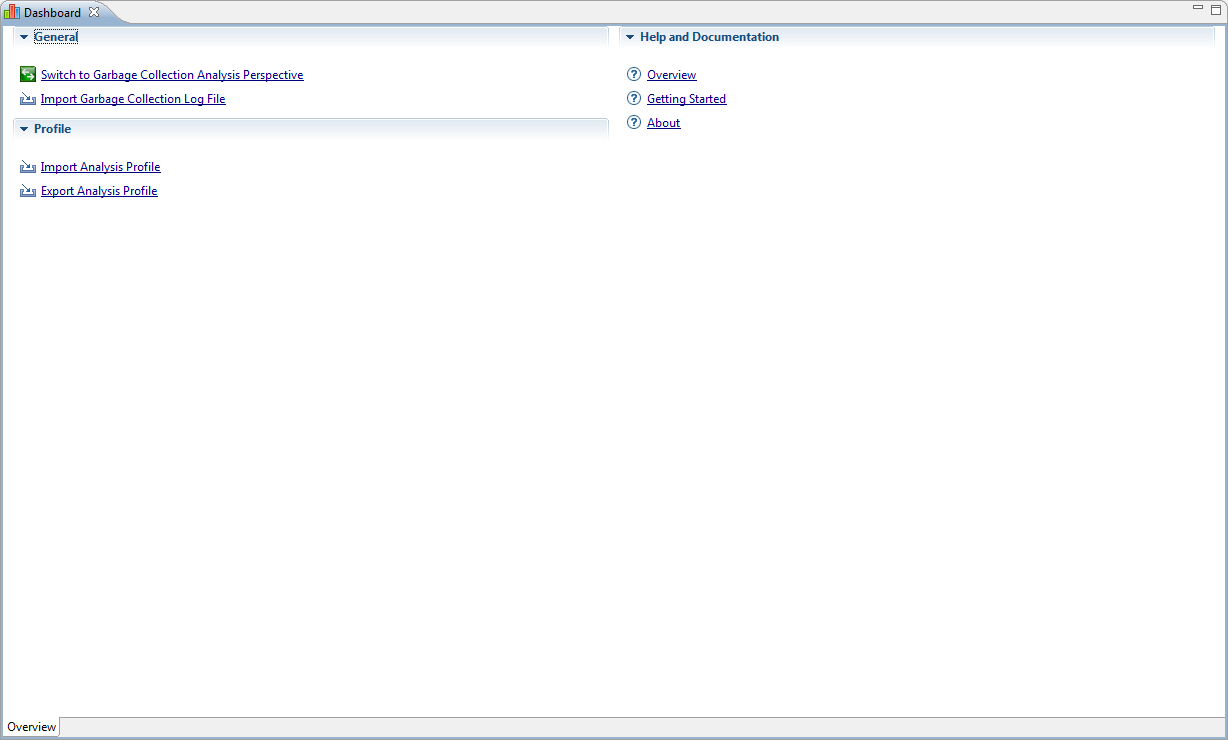
\includegraphics[width=16cm]{images/tutorial_dashboard}
        	\caption{Dashboard}
\end{figure}

Auf dem Dashboard befinden sich verschiedene Sektionen mit unterschiedlichen Funktionen:
\begin{itemize}
	\item Sektion General 
		\begin{itemize}
			\item Wechsel in die Garbage Collection Perspektive
			\item Import einer Garbage Collection Log Datei
		\end{itemize}
	\item Sektion Profile
		\begin{itemize}
			\item Import eines Analyseprofils
			\item Export eines Analyseprofils
		\end{itemize}
	\item Sektion Help and Documentation
		\begin{itemize}
			\item Beinhaltet Links auf verschiedene Inhalte der Hilfe
		\end{itemize}
\end{itemize}

\section{Import einer Garbage Collection Log Datei}
Der Import-Dialog kann auf verschiedene Arten geöffnet werden:
\begin{itemize}
	\item Über die View Log Dateien mit Rechsklick / Import Garbage Collection Log File.
	\item Über File / Import / Import Garbage Collection File (Kategorie: Garbage Collection)
	\item Im Dashboard über Import Garbage Collection Log File
\end{itemize}

Über den Browse Button muss der Ordner angegeben werden, der die Log-Dateien beinhaltet, anschliessend kann die Log-Datei im darunterliegenden Fenster selektiert werden. Mit Klick auf Finish wird die Datei importiert.
 \begin{figure}[H]
  	\centering
    	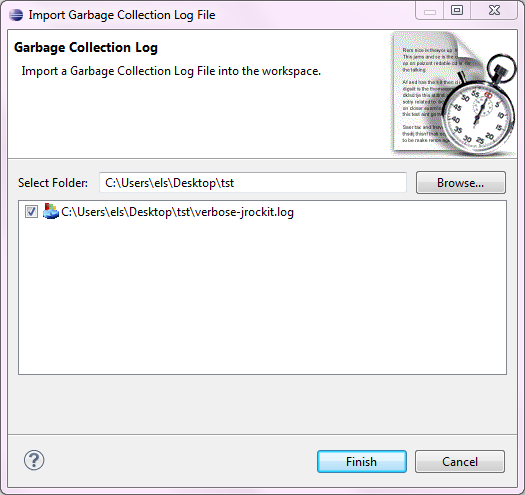
\includegraphics[width=10cm]{images/tutorial_importlog}
        	\caption{Import Wizard}
\end{figure}

\section{Profile}
Zur Verwaltung der verschiedenen Analyseprofile gibt es die View Profiles. In ihr können Profile erstellt, exportiert und importiert werden. Wenn eine Log-Datei mit einem bestimmten Analyseprofil geöffnet werden soll, muss das entsprechende Profil darüber aktiviert / selektiert werden.

\subsection{Profil erstellen}
Mit Rechtsklick auf die Profiles View / Create Profile oder File / New / Other... / Analysis Profile (Kategorie Garbage Collection) kann der Dialog zum erstellen eines neuen Profils geöffnet werden. 
 \begin{figure}[H]
  	\centering
    	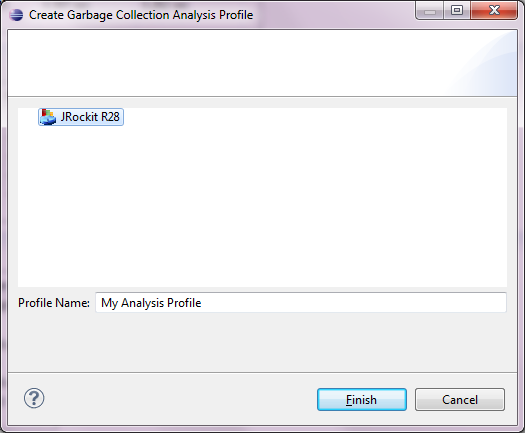
\includegraphics[width=10cm]{images/tutorial_newprofile}
        	\caption{Profil erstellen}
\end{figure}
Mit der Bedingung, dass ein Log-Format selektiert wurde (im Beispiel JRockit R28) und ein Namen vergeben wurde, wird ein neues Profil in der Profiles View erstellt.

\subsection{Profil exportieren}
Mit Rechtsklick auf die Profiles View / Export Profile können die Profile in eine Lap\footnote{Lap steht für Log Analysis Profile}-Datei exportiert werden.
 \begin{figure}[H]
  	\centering
    	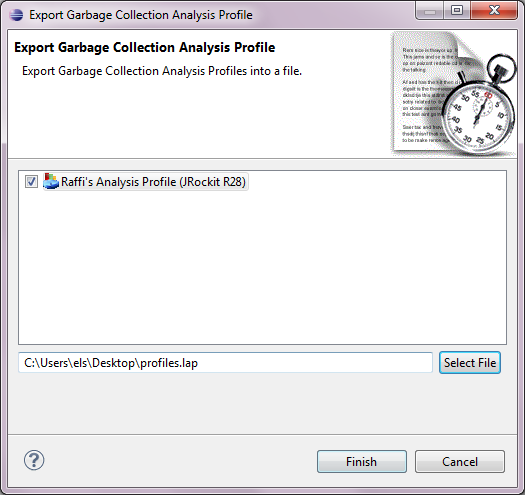
\includegraphics[width=10cm]{images/tutorial_exportprofile}
        	\caption{Profil exportieren}
\end{figure}

\subsection{Profil importieren}

Mit Rechtsklick auf die Profiles View / Import Profile können die Profile aus einer Lap-Datei importiert werden.
 \begin{figure}[H]
  	\centering
    	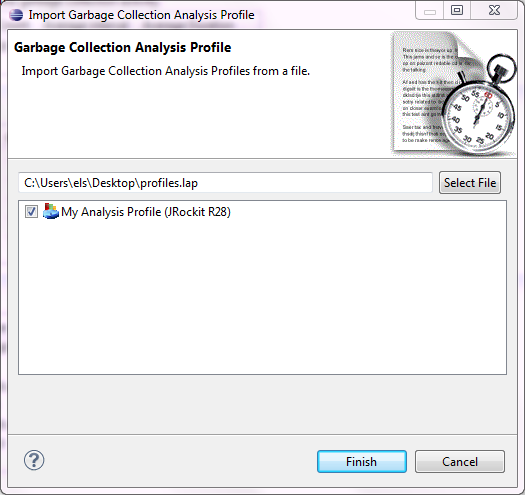
\includegraphics[width=10cm]{images/tutorial_importprofile}
        	\caption{Profil importieren}
\end{figure}

\section{Garbage Collection Analyse}
\subsection{Standardauswertung}
Sofern in der Profiles Ansicht kein Profil oder das Standard Profil selektiert ist, wird mit Doppelklick auf die importierte Log Datei in der Log Files Ansicht die Standardauswertung geöffnet. Die Standardauswertung besteht aus drei unterschiedlichen Tabs. Der erste Tab zeigt eine Zusammenfassung der Garbage Collection, der zweite Tab den Verlauf des benötigten Speichers auf dem Heap, und der dritte Tab die Dauer der einzelnen Garbage Collection Zyklen. 

\subsubsection{Zusammenfassung}
 \begin{figure}[H]
  	\centering
    	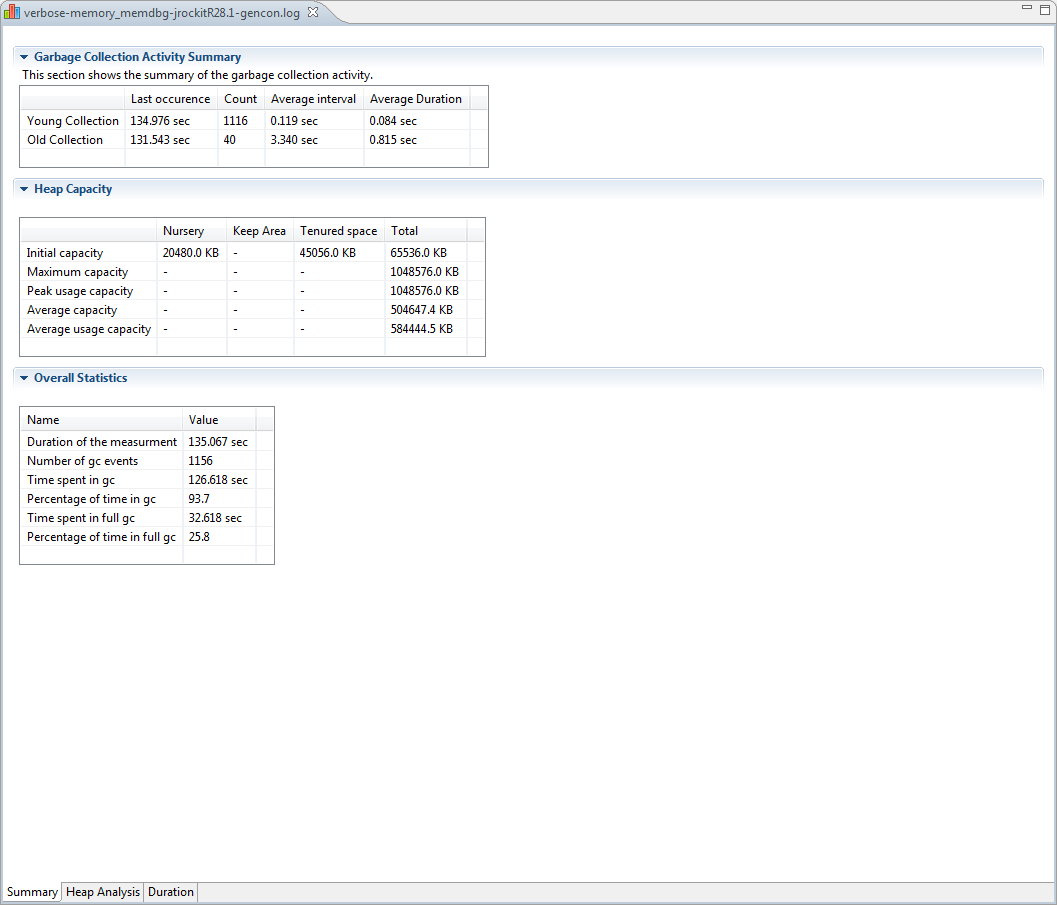
\includegraphics[width=15cm]{images/tutorial_standardreport_statistics}
        	\caption{Standardauswertung: Zusammenfassung}
\end{figure}

\subsubsection{Heap Analyse}
 \begin{figure}[H]
  	\centering
    	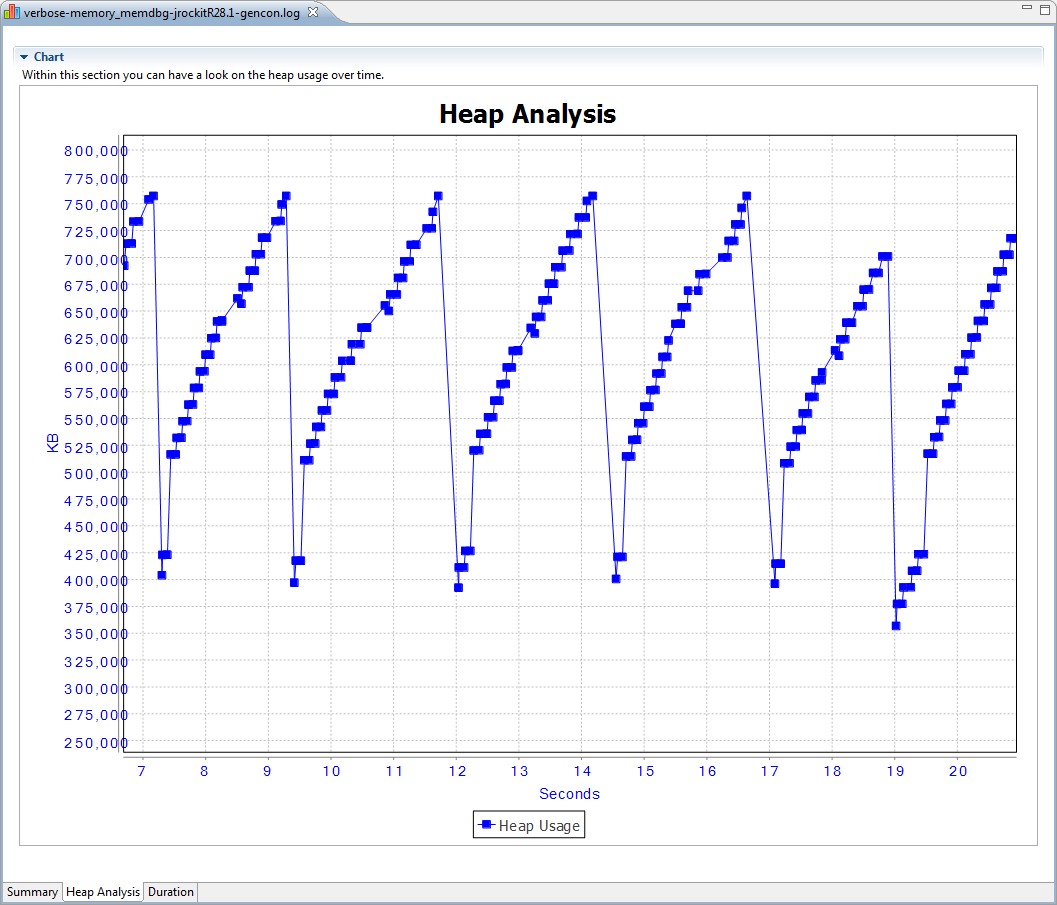
\includegraphics[width=15cm]{images/tutorial_standardreport_heapanalysis}
        	\caption{Standardauswertung: Heap Analyse}
\end{figure}

\subsubsection{Dauer Garbage Collection}
 \begin{figure}[H]
  	\centering
    	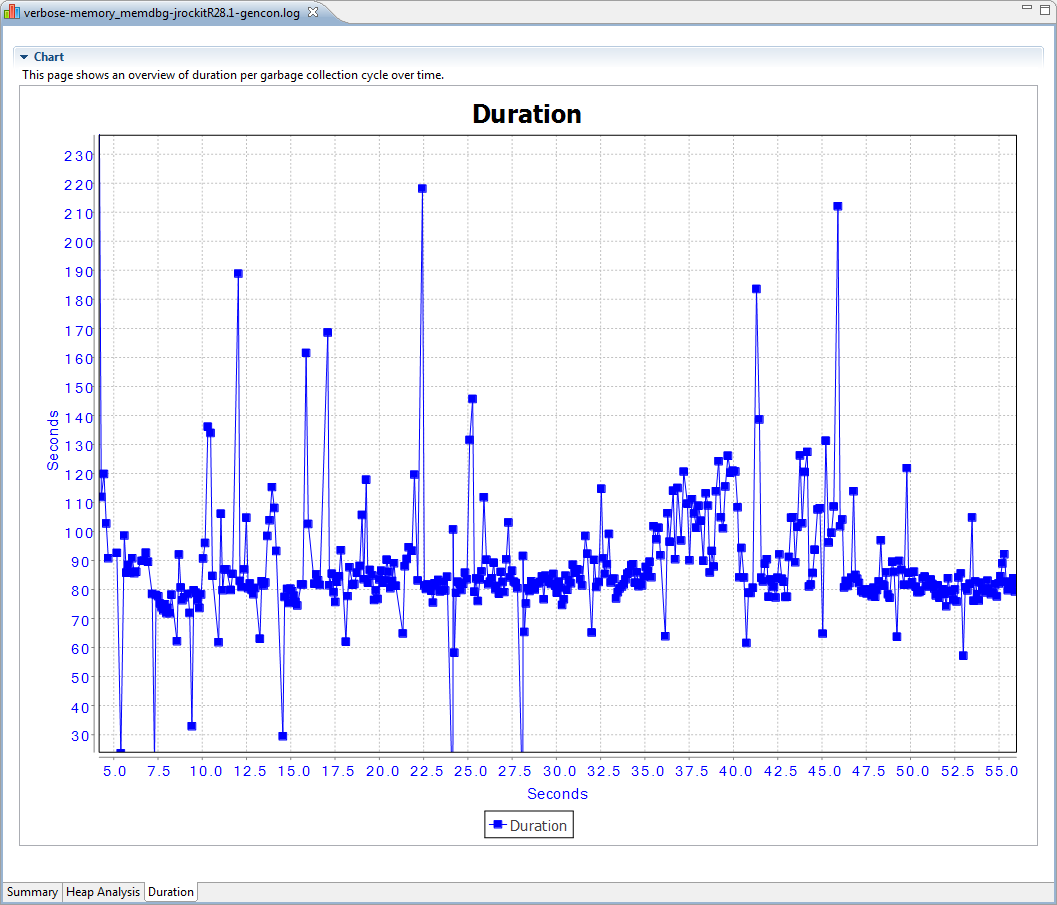
\includegraphics[width=15cm]{images/tutorial_standardreport_duration}
        	\caption{Standardauswertung: Dauer Garbage Collection}
\end{figure}



\subsection{Benutzerdefinierte Auswertung (Profile)}
Die benutzerdefinierte Auswertung wird geöffnet, indem man vor dem öffnen einer Datei ein zuvor erstelltes Profil selektiert. 
 \begin{figure}[H]
  	\centering
    	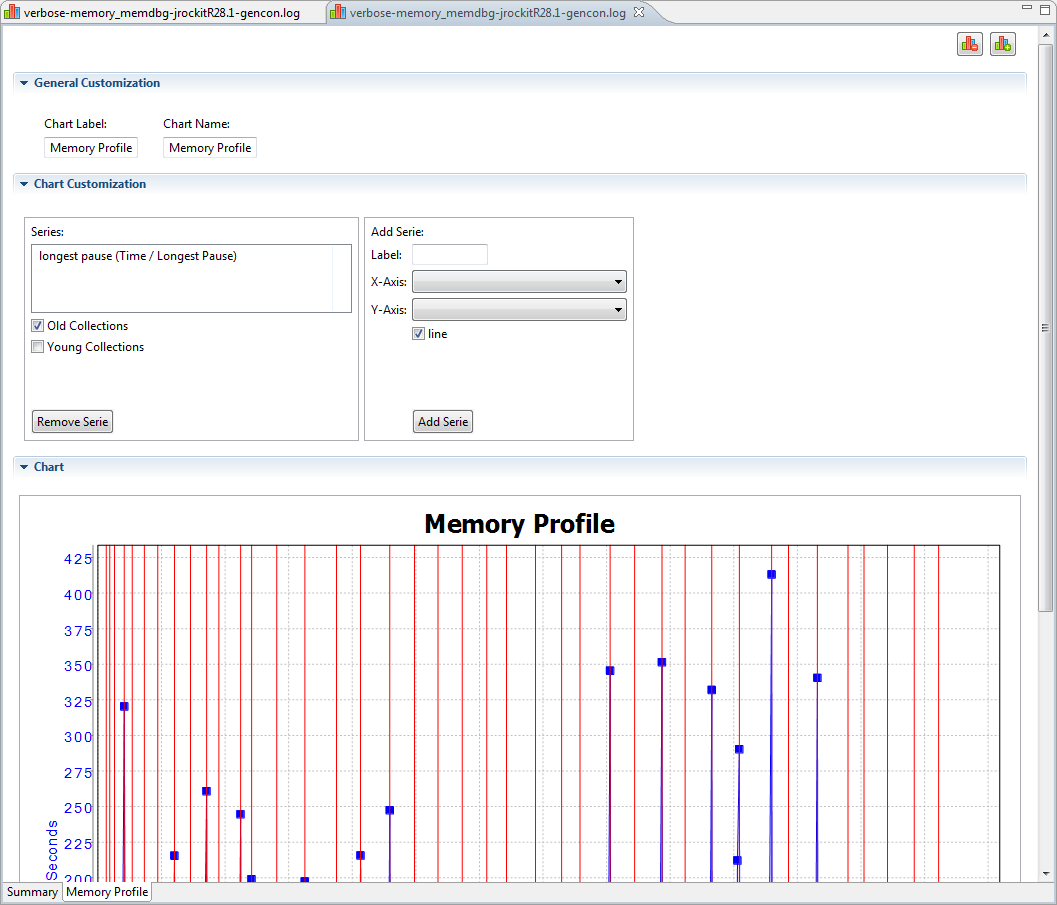
\includegraphics[width=15cm]{images/tutorial_custom_report}
        	\caption{Standardauswertung: Zusammenfassung}
\end{figure}
Im Abschnitt General Customization können die Namen des Tabas und des Charts definiert werden. Im Abschnitt Chart Customization können neue Serien auf das Chart hinzugefügt werden. Dabei können pro Serie die Werte für die X-, Y-Achse angegeben werden, der Name der Serie definiert und angegeben werden, ob die Punkte der Serie mit einer Linie verbunden werden sollen. Die Ende der Garbage Collection können als vertikale Linien in rot (Old Collections) oder blau (Young Collections) angezeigt werden.

